\newpage
\section{Session Experiment - Results} \label{sec:lv_session_results}
In this section we will test the estimation process carried by the Laplace Transform estimator presented in Section \ref{sec:laplace_estimator} in addition with the Kolmogorov-Smirnov validation test for different session cases.

We generated a traffic configuration that gave us a load of 30-35\% for 20 users in order to be used as a fixed configuration for all the experiments. In this case, we will fix the flow number and flow inter-arrival for each session, randomizing flow sizes, packet sizes and packet inter-arrival. Using the chosen traffic configuration, we will decrease only the number of users to have four different session cases: 20, 15, 10 and 5 \acs{WLAN} users. The user realizations for each session case is represented in Figure \ref{fig:lv_user_realization}. Each one of these session-cases will represent a different load case. We run 200 runs for each session case. The traffic configuration for these experiments is presented in Table \ref{table:lv_traffic}.

\begin{figure}[h!]
	\centering
	\subfloat[5 sessions - 3 sensors]{
		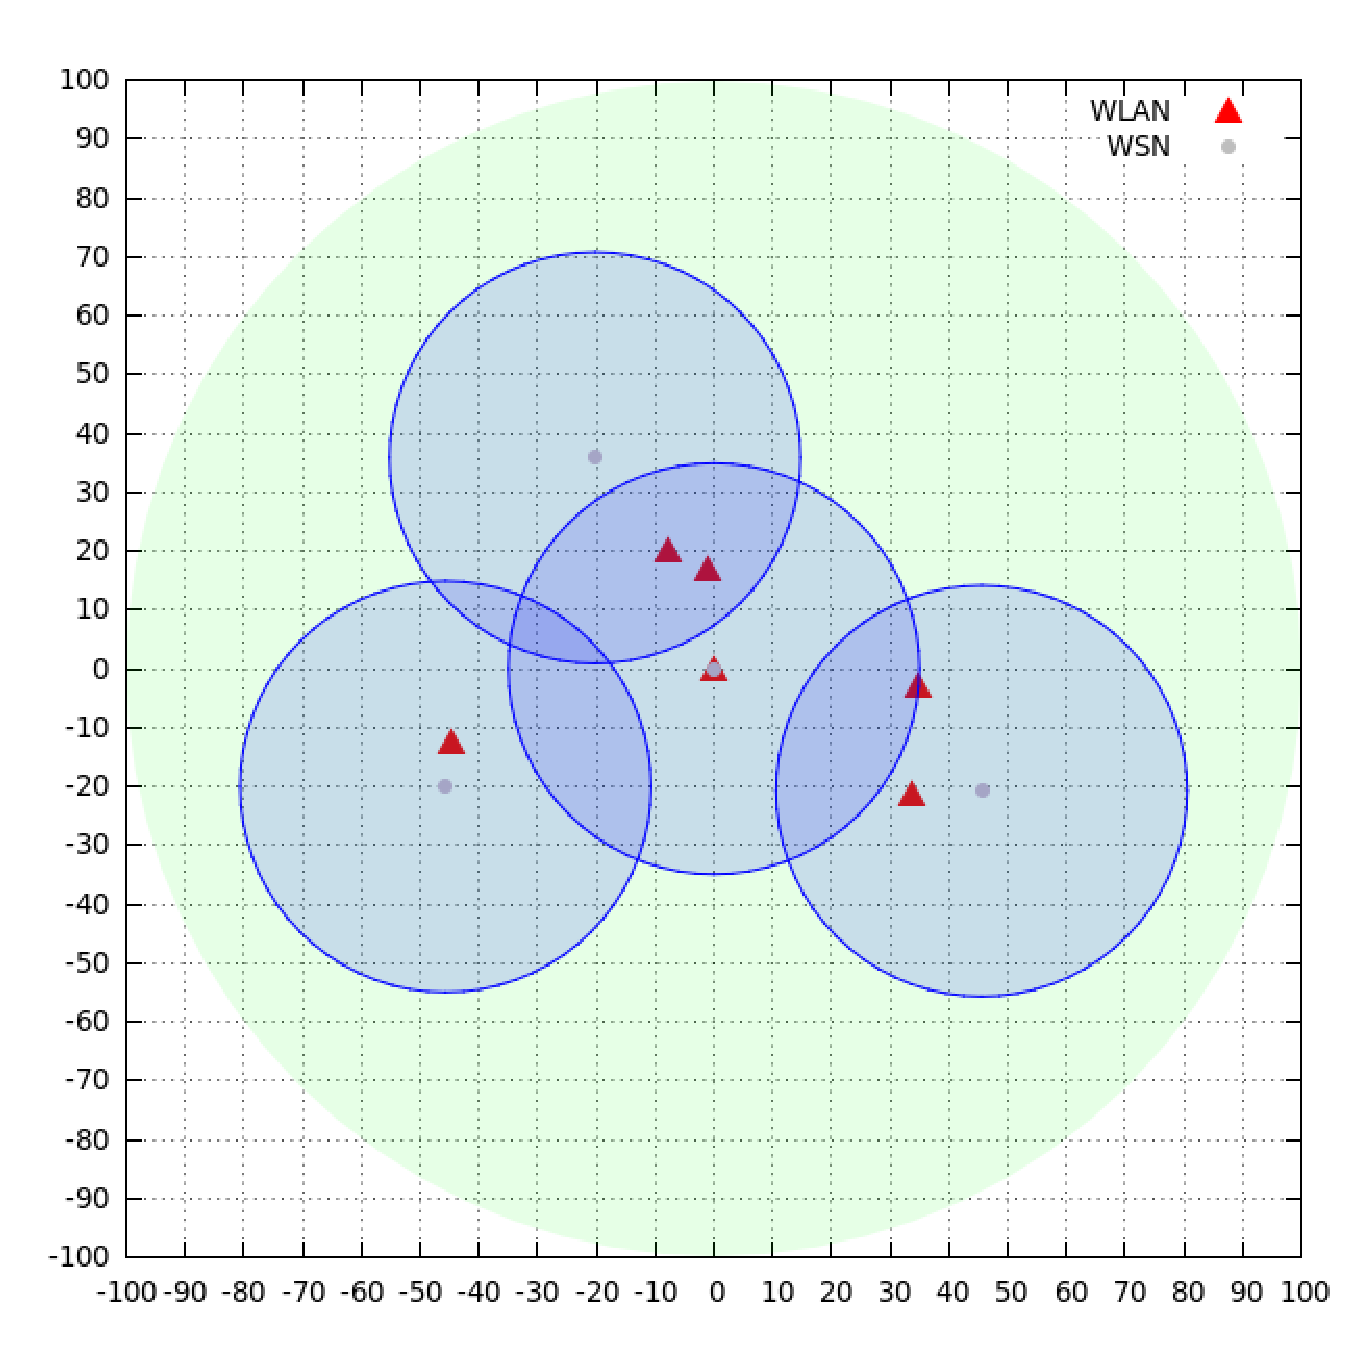
\includegraphics[width=0.25\textwidth]{images/results/localview/session_experiment/5sessions_3sensors}
	}
	\subfloat[10 sessions - 3 sensors]{
		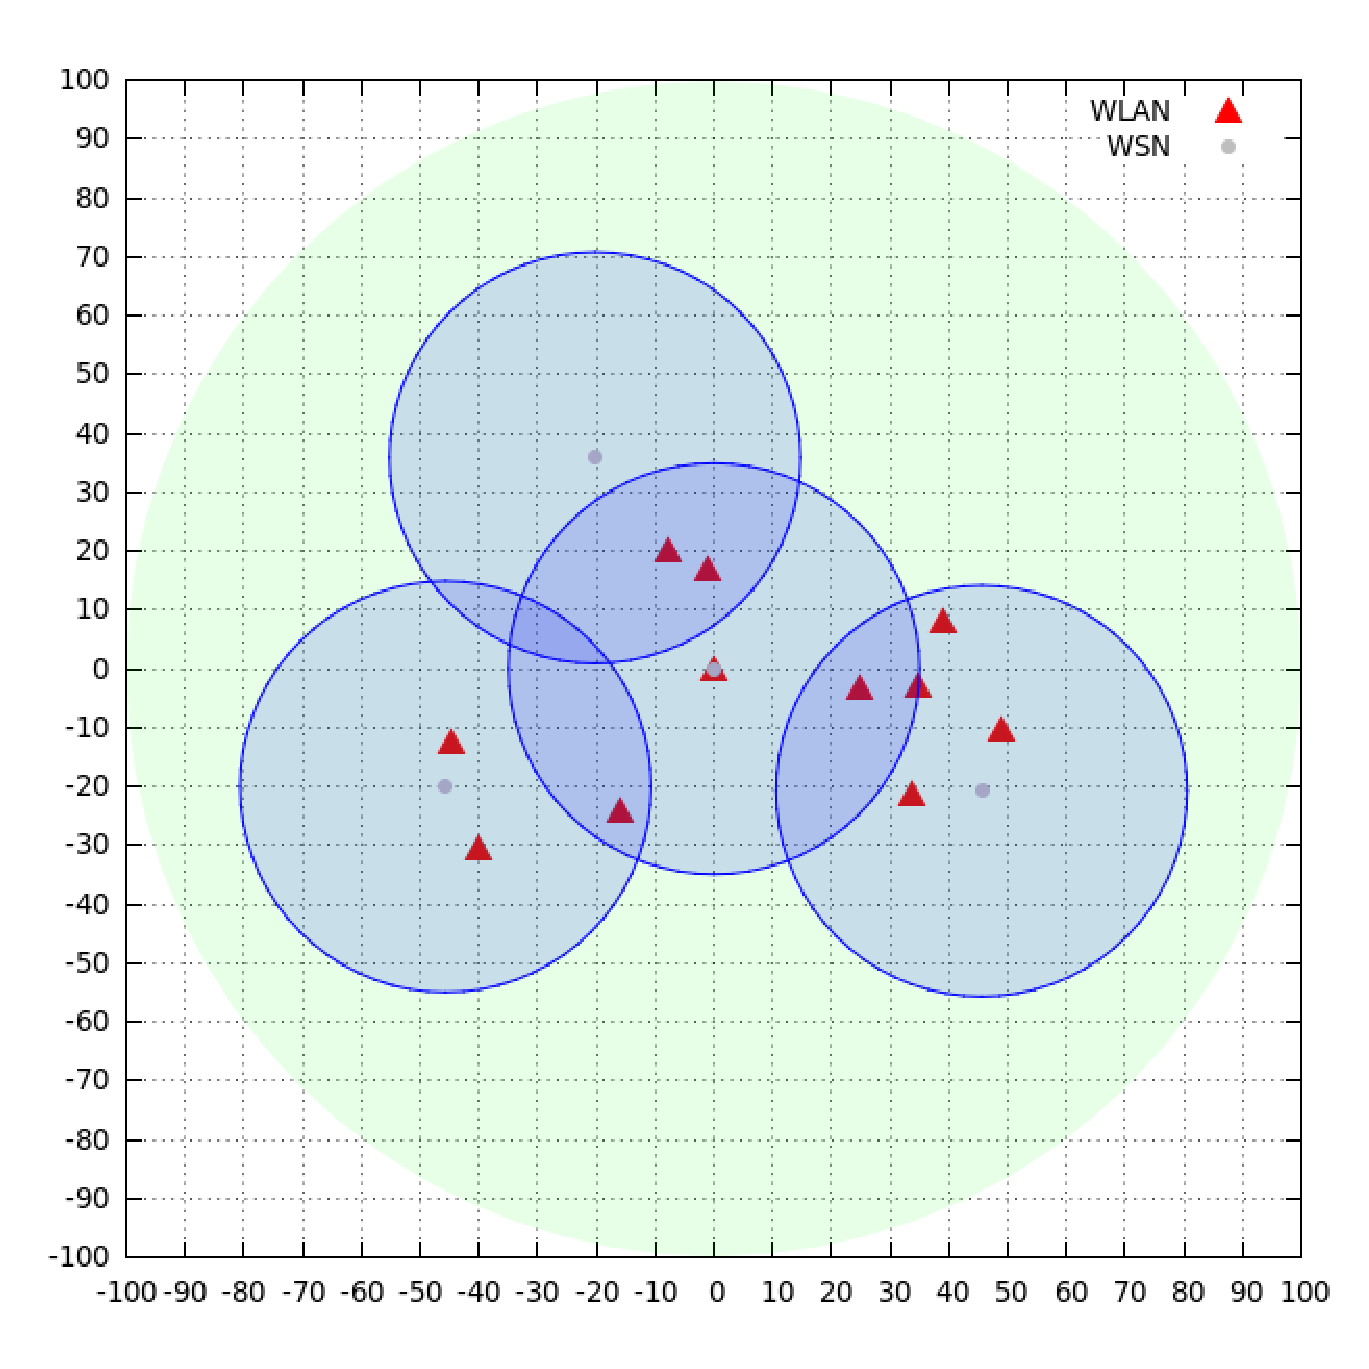
\includegraphics[width=0.25\textwidth]{images/results/localview/session_experiment/10sessions_3sensors}
	}
	\subfloat[15 sessions - 5 sensors]{
		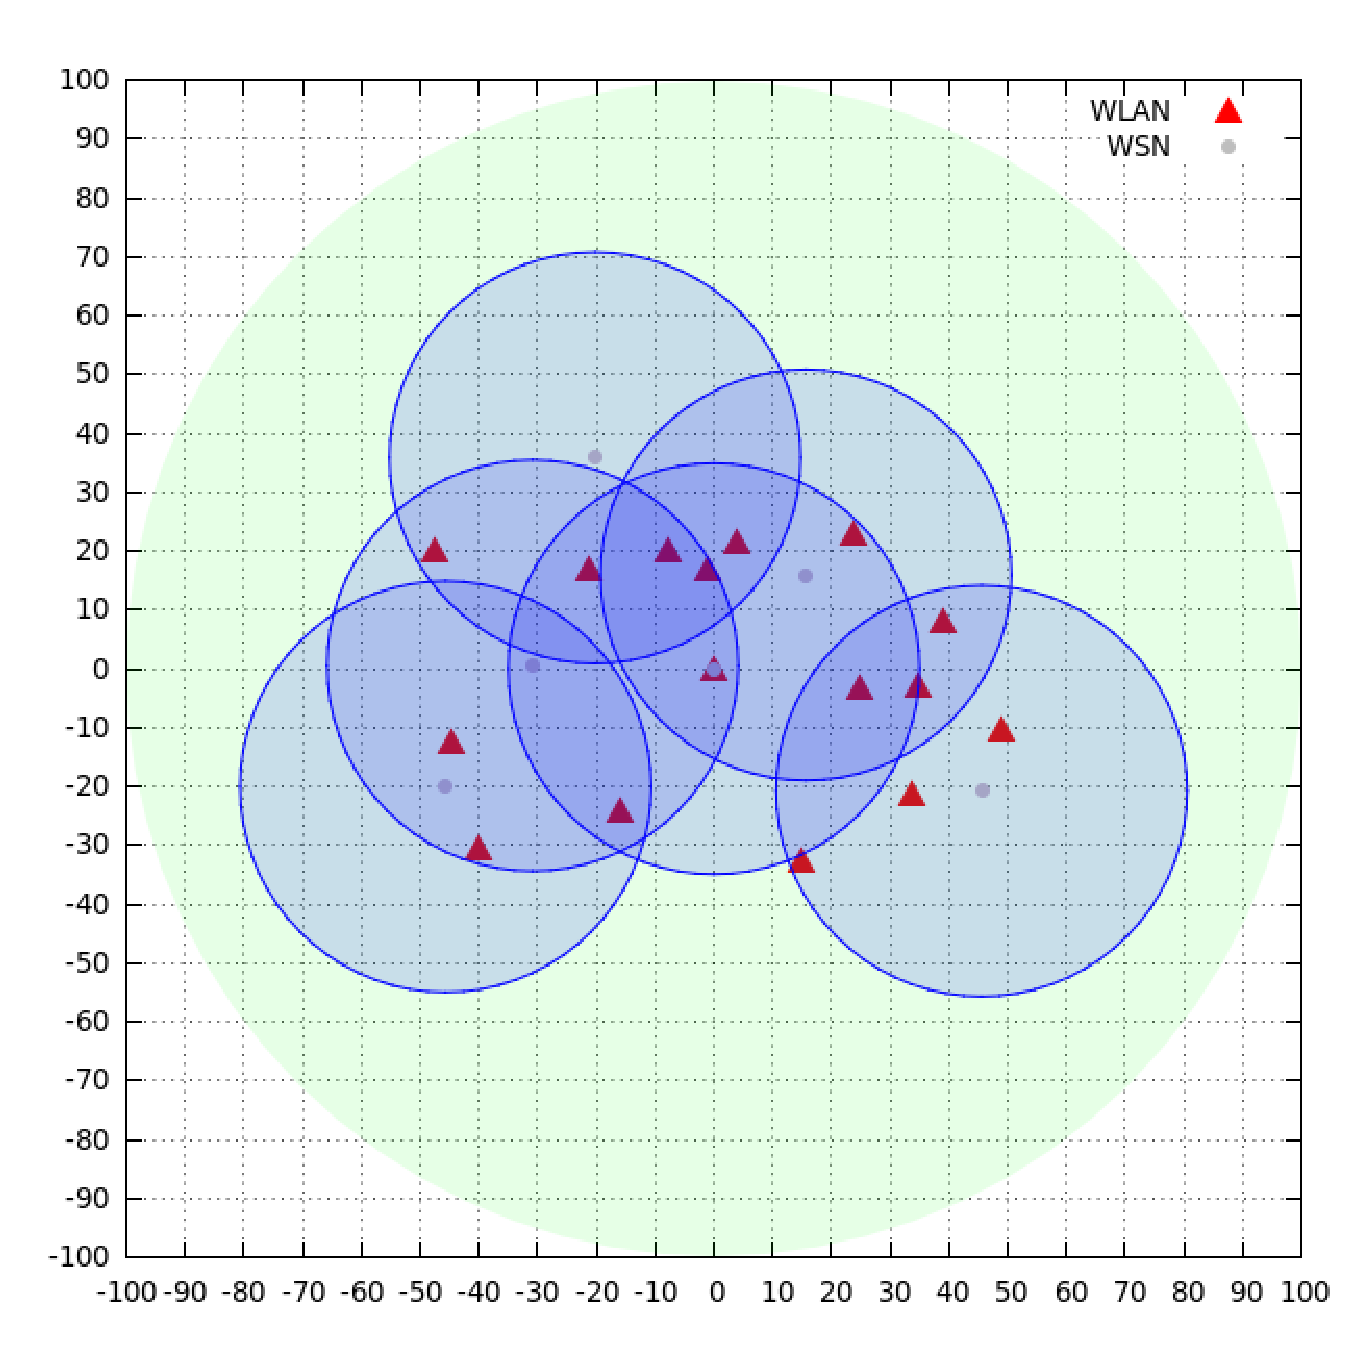
\includegraphics[width=0.25\textwidth]{images/results/localview/session_experiment/15sessions_5sensors}
	}
	\subfloat[20 sessions - 5 sensors]{
		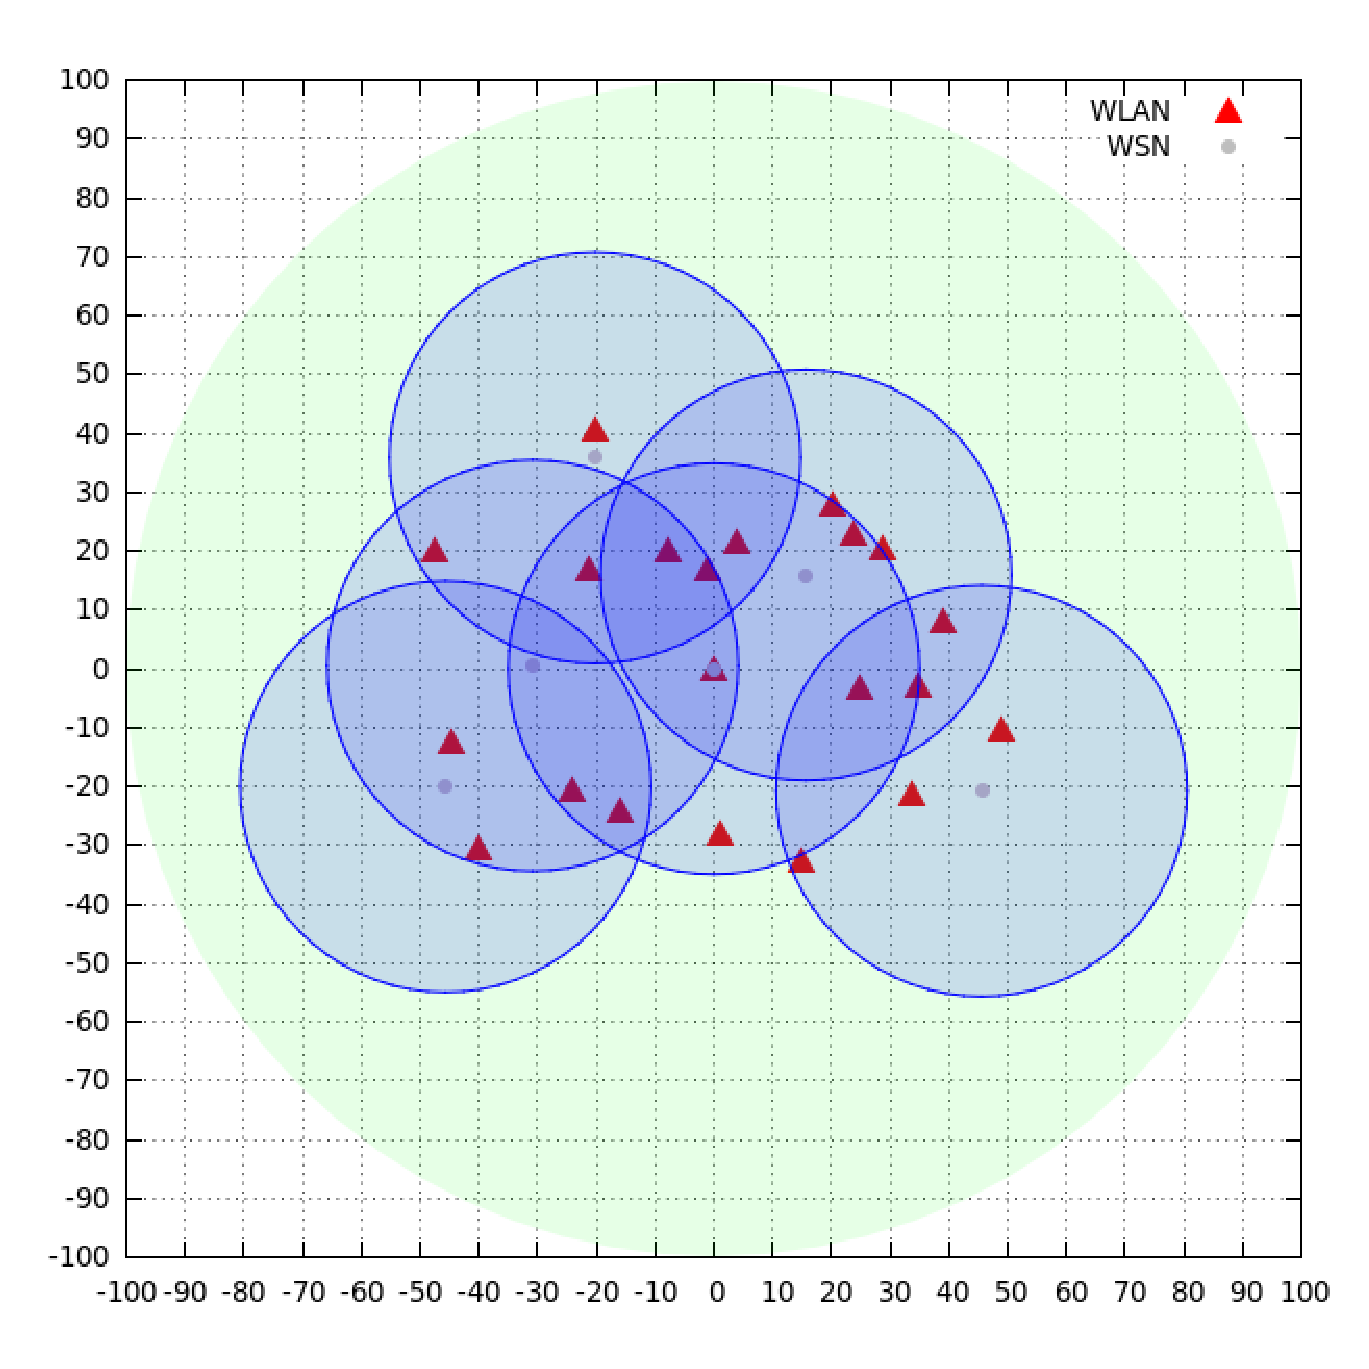
\includegraphics[width=0.25\textwidth]{images/results/localview/session_experiment/20sessions_5sensors}
	}
	\caption{User realization for the Local View session experiment}
	\label{fig:lv_user_realization}
\end{figure}

\begin{table}[h!]
	\begin{center}
		\begin{tabular}{ l | c | c | c }
			Modeled Variable & Distribution & Parameters & \\ \hline
			Session number	& Fixed & N users arriving at simulator start \\
			Flow inter-arrival & Log-normal & $\mu = -1.6355$, $\sigma = 2.6286$ & fixed\\
			Flow number & Bi-Pareto & $\alpha = 0.07$, $\beta = 1.75$, $c = 295.38$, $k = 1$ & fixed\\
			Flow Size & Bi-Pareto & $\alpha = 0.00$, $\beta = 1.02$, $c = 15.56$, $k = 111$ & random\\
			Packet Size & Uniform & $min = 512$, $max = 1024$ & random\\
			Packet inter-arrival & Exponential & $\lambda = 10$ & random\\
		\end{tabular}
		\caption{Traffic configuration for the Local View session experiment according to \cite{Campus-WLAN}.}
		\label{table:lv_traffic}
	\end{center}
\end{table}

The experiment will be done as follows: for each run of simulation, considering a Global View model, a sensor will estimate the parameters and the Kolmogorov-Smirnov validation test for the Global View model. If the validation test is successful ($p-value > 0.05$), then each sensor, considering now the Local View model, will perform the Laplace Transform estimation with the samples gathered from the users within range and extract the parameters for the local active and idle distributions.

Table \ref{table:lv_session_exp_ks} shows the pass-rate of the \acs{K-S} test for this experiment. As it can be observed, for the low-load cases, the \acs{K-S} fail rate is quite high. On the other hand, this behaviour is not present in the medium and high load cases (15 and 20 session respectively).

\begin{table}[h!]
	\centering
	\begin{tabular}{ c | c }
		& $P(p-value < 0.05)$ \\ \hline
		5 sessions &  78.5 \%\\ 
		10 sessions & 26 \% \\
		15 sessions & 0 \% \\
		20 sessions & 3,97 \%
	\end{tabular}
	\caption{\acs{K-S} failure rate for the Local View session experiment (over 200 runs)}
	\label{table:lv_session_exp_ks}
\end{table}

The results of the estimation for this experiment are represented in Figures \ref{fig:lv_session_exp1} and \ref{fig:lv_session_exp2}. These figures represent only the results after the \acs{K-S} filtering. Each one of the sub-figures represent each one of the estimated parameters (mean and deviation) for each one of the sensors in addition with the Global View estimated values. In these sub-plots, we represented the estimated parameters for the tests that passed previously the \acs{K-S}.

\begin{figure}[h!]
	\centering
	\subfloat[5 sessions (Load range: 8-10\%)]{
		\label{fig:lv_5_sessions}
		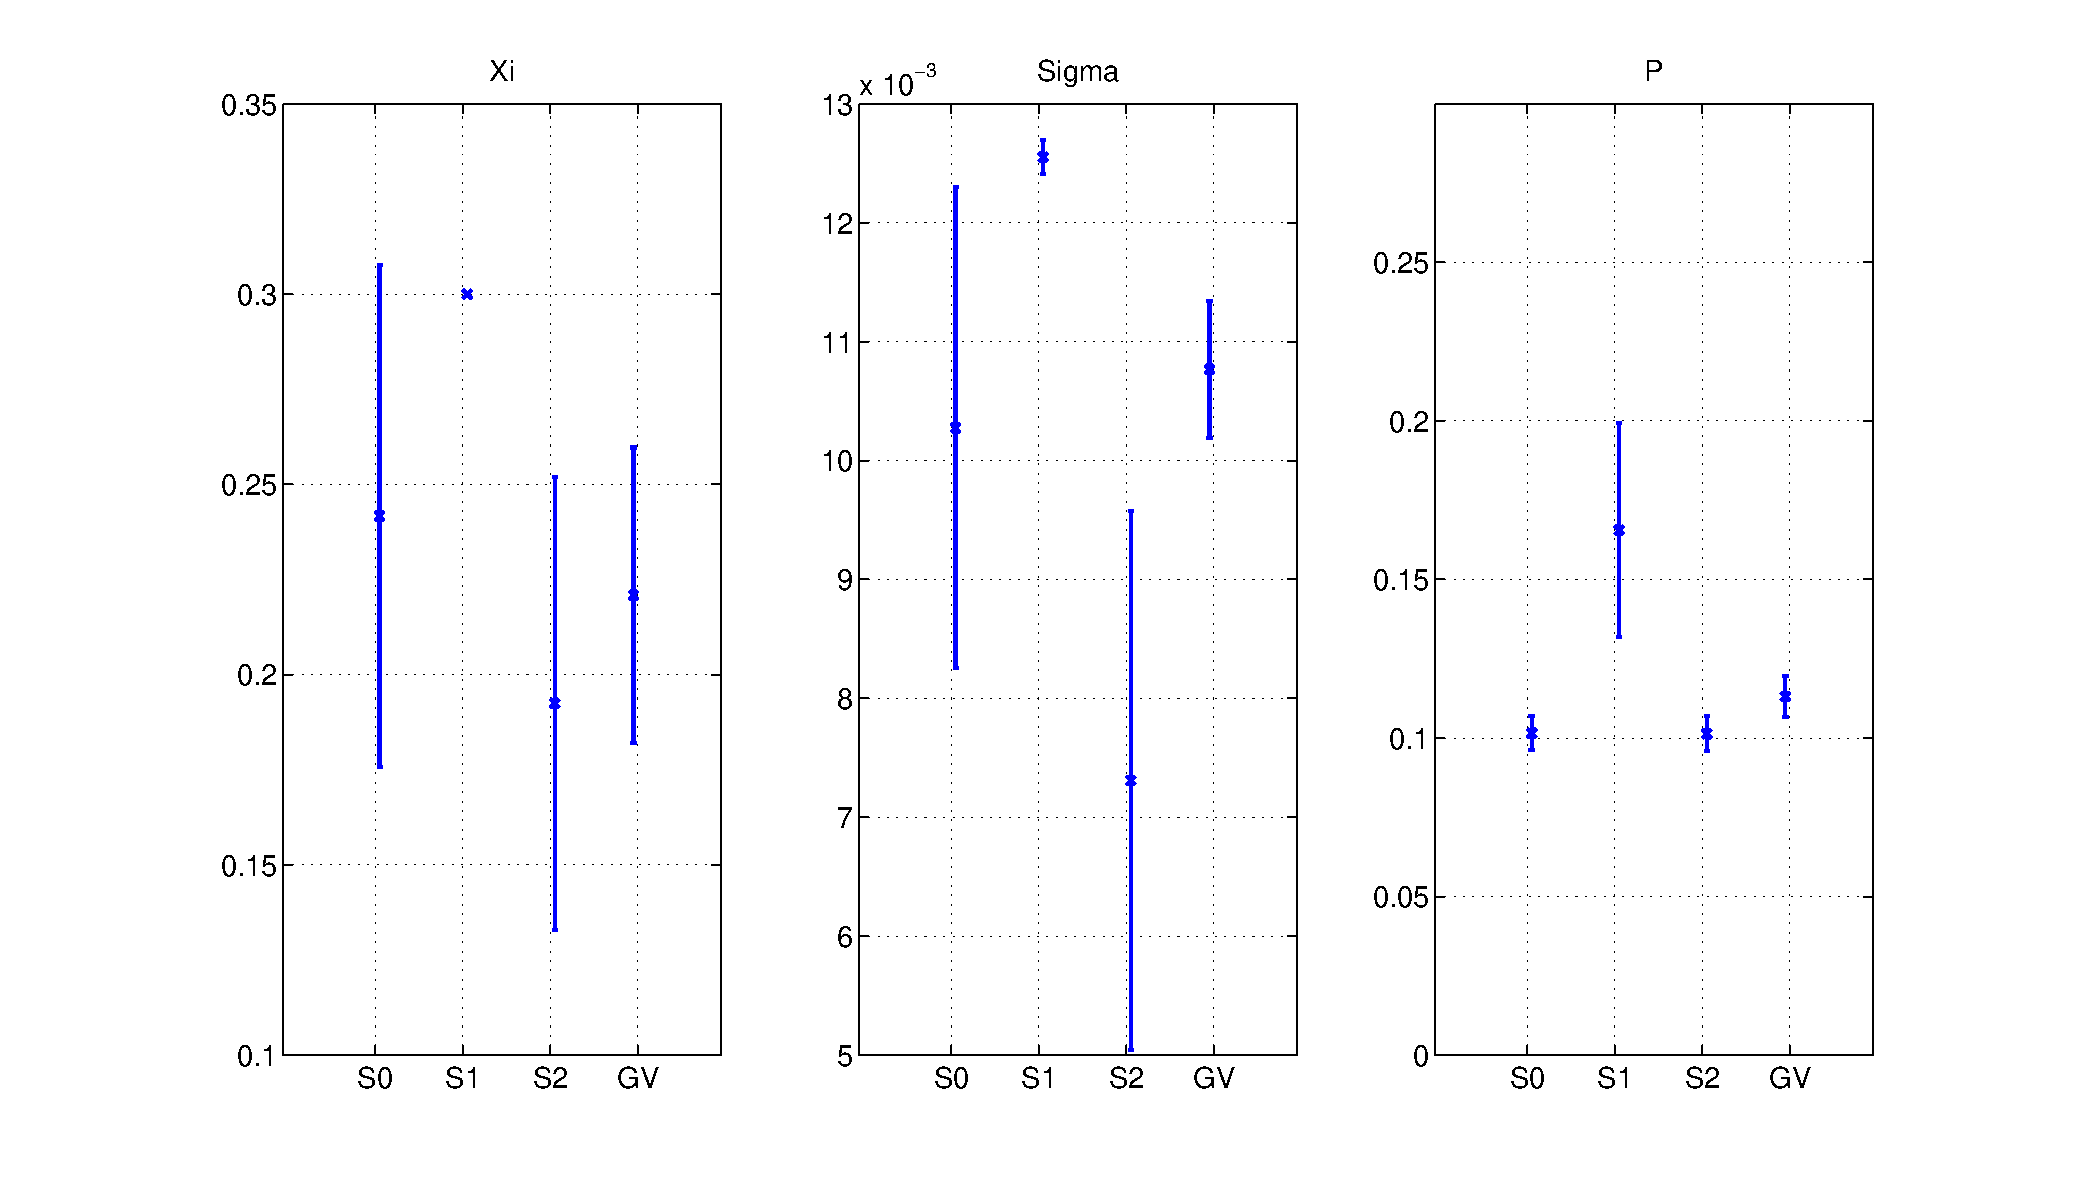
\includegraphics[width=1\textwidth]{images/results/localview/session_experiment/5sessions}
	}\\
	\subfloat[10 sessions (Load range: 12-15\%)]{
		\label{fig:lv_10_sessions}
		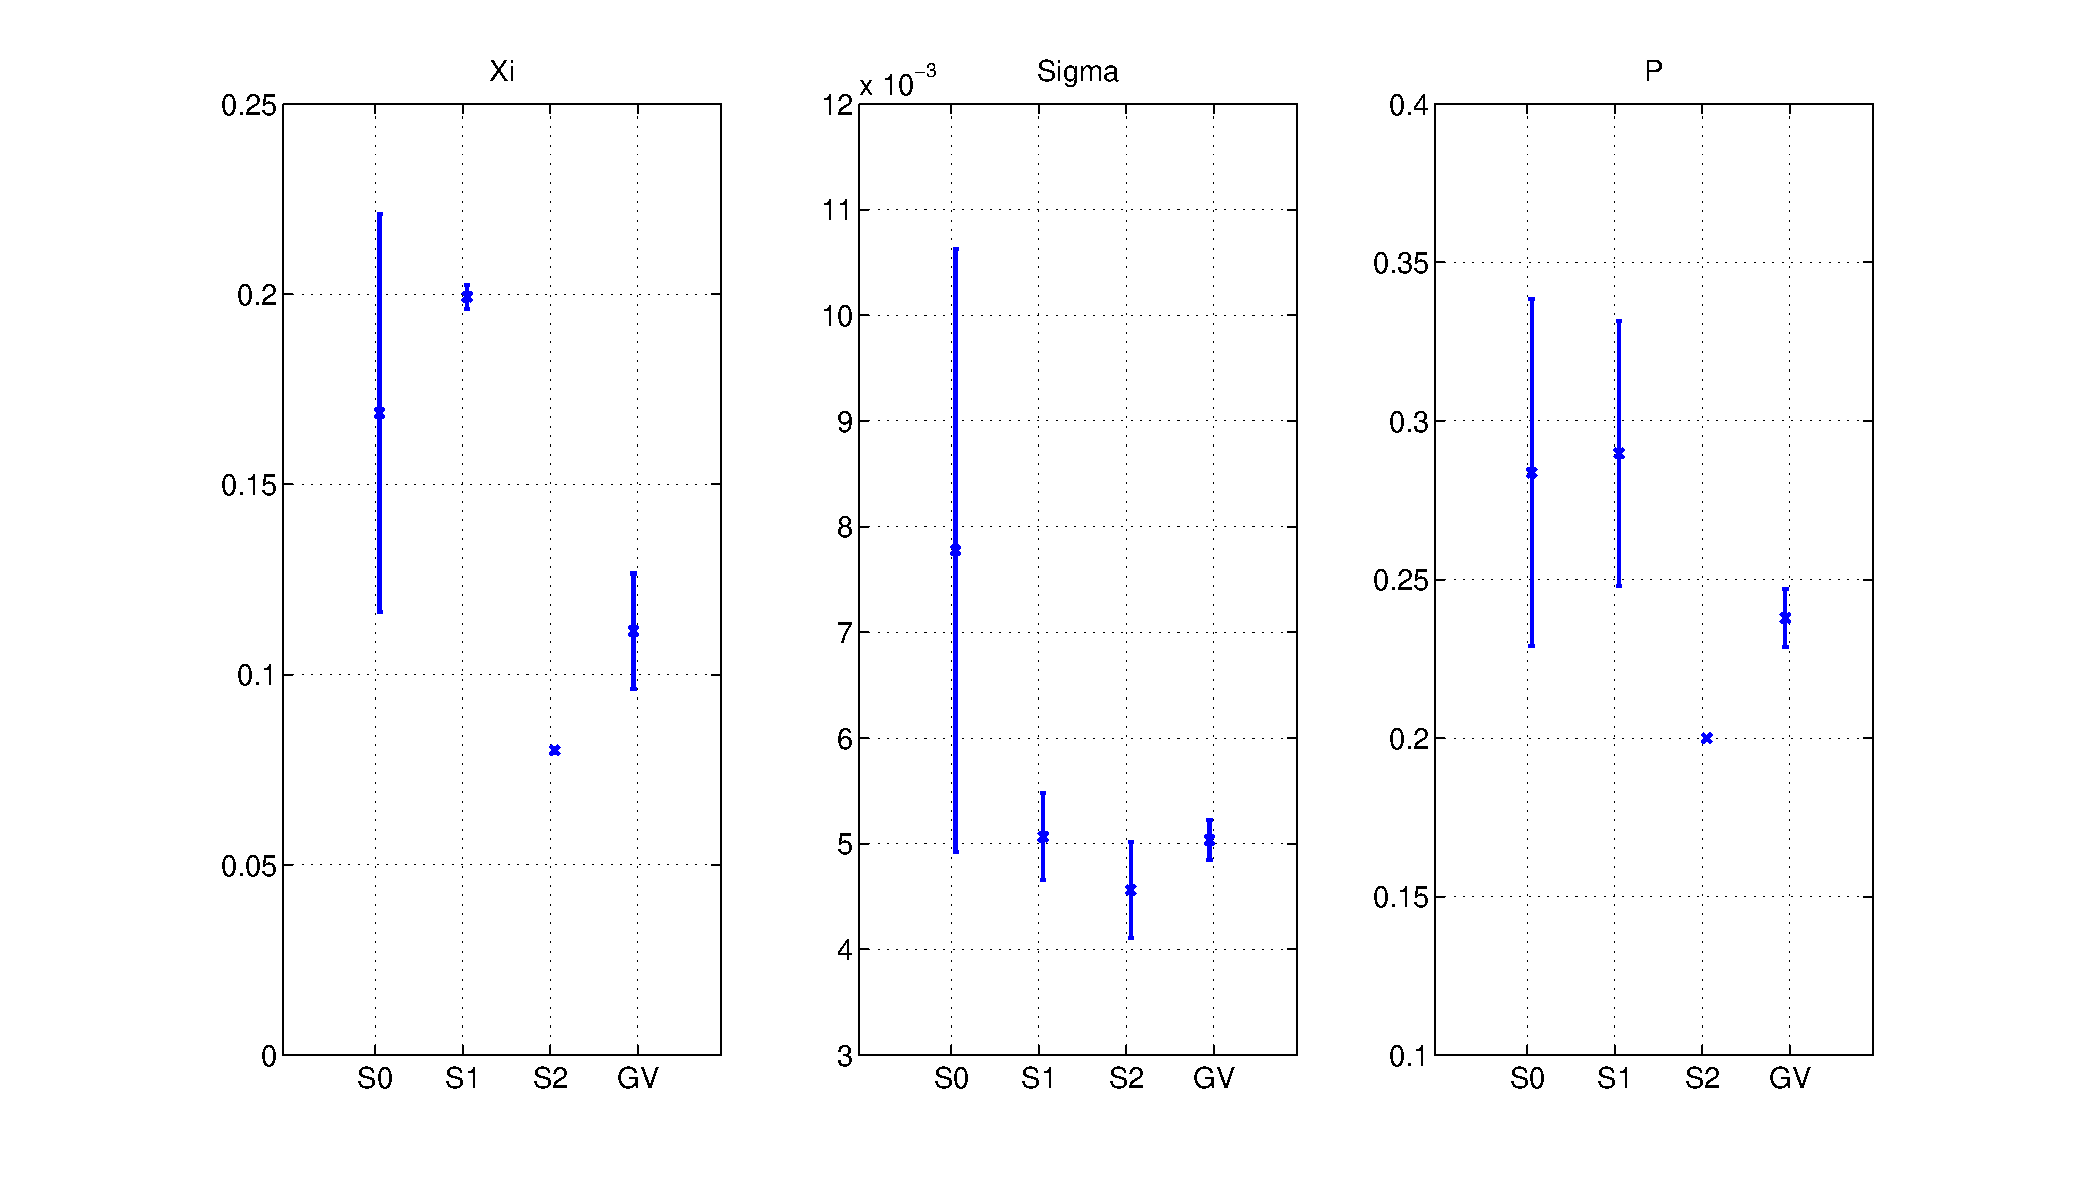
\includegraphics[width=1\textwidth]{images/results/localview/session_experiment/10sessions}
	}
	\caption{Session experiment for the Local View model (I). Different session cases using the same traffic configuration for flow number and flow inter-arrivals.}
	\label{fig:lv_session_exp1}
\end{figure}

\begin{figure}[h!]
	\centering
	\subfloat[15 sessions (Load range: 20-25\%)]{
		\label{fig:lv_15_sessions}
		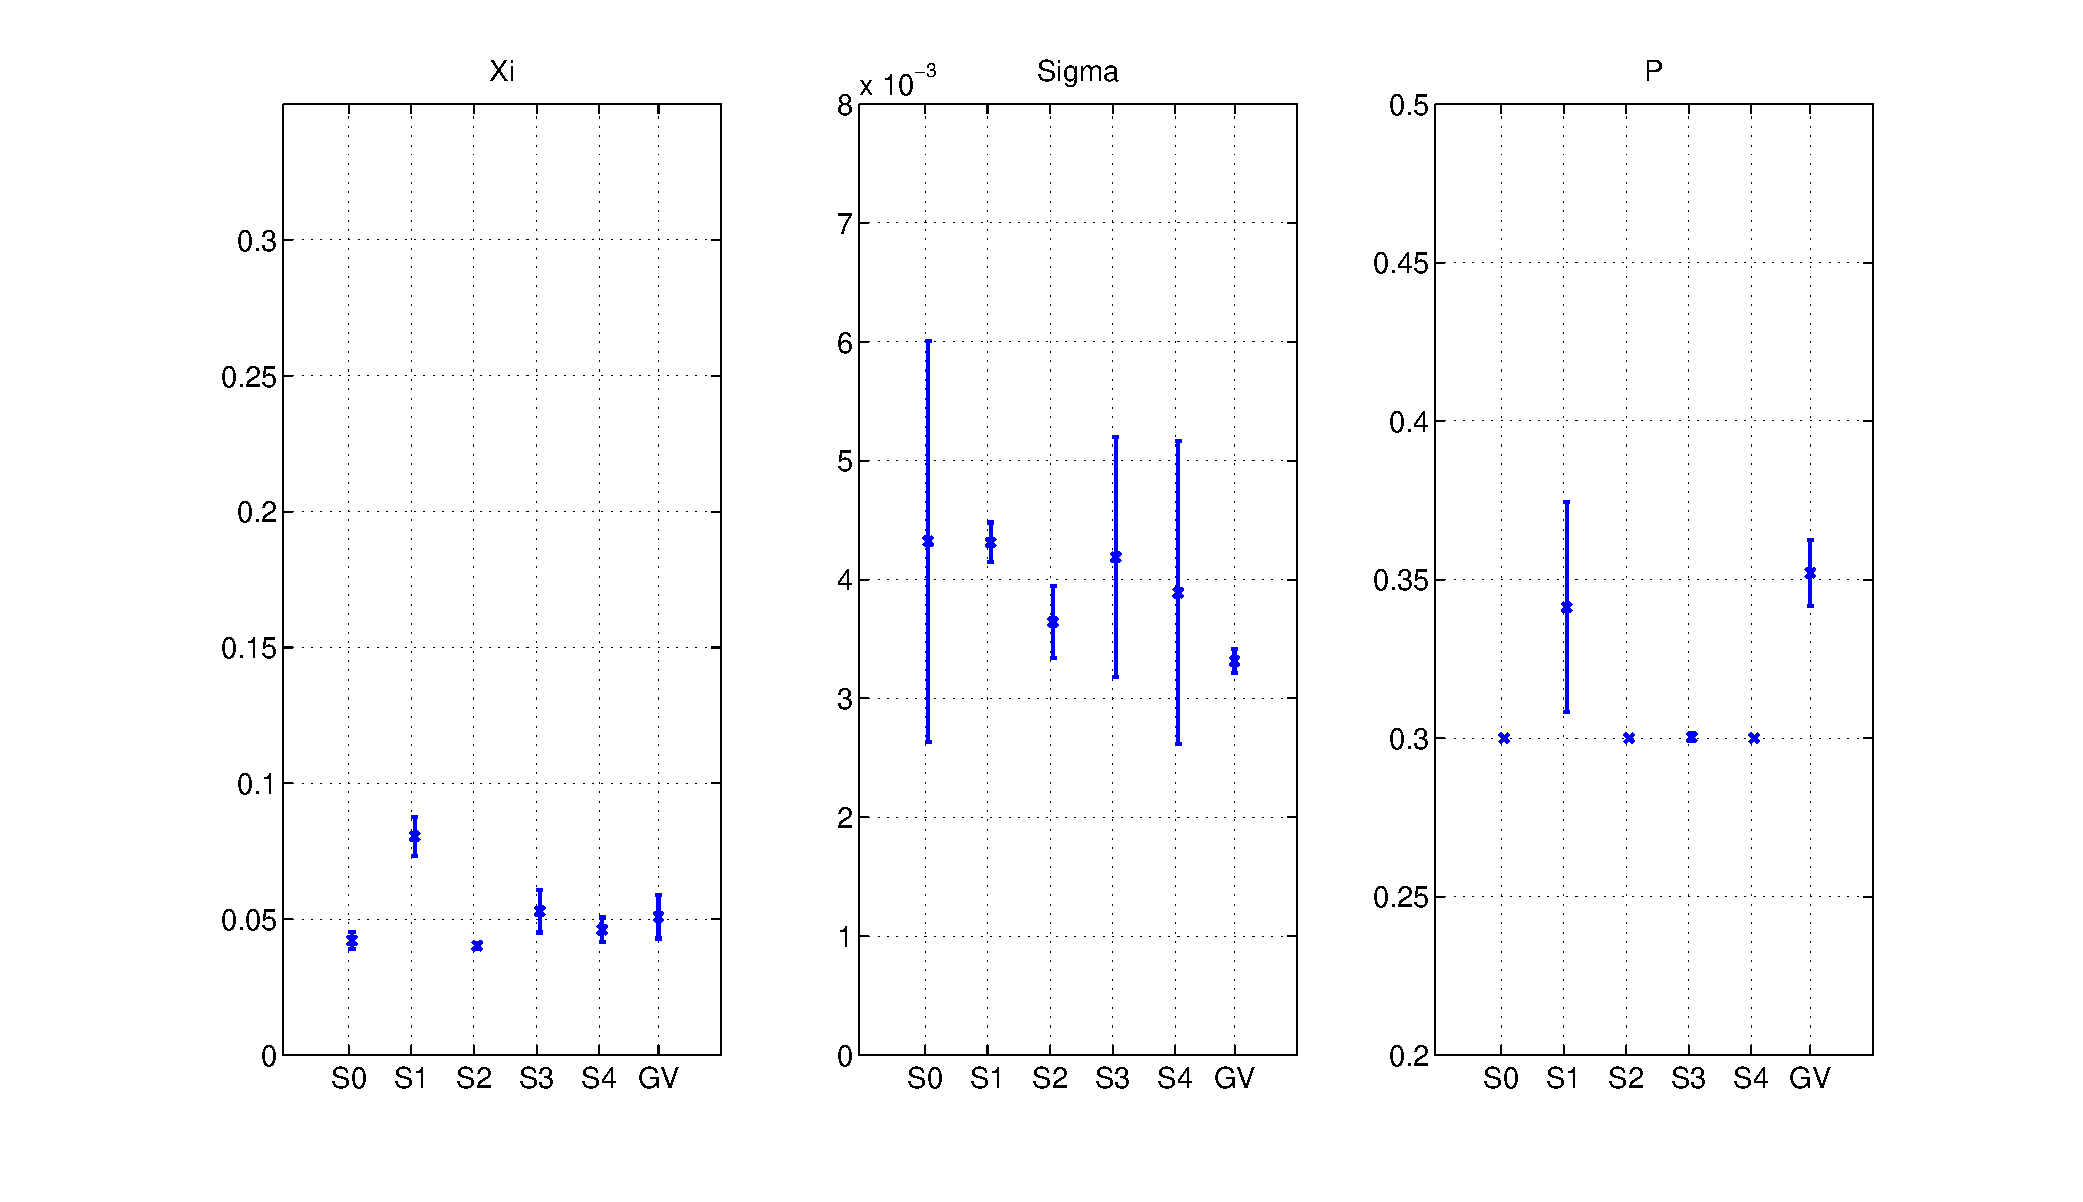
\includegraphics[width=1\textwidth]{images/results/localview/session_experiment/15sessions}
	}\\
	\subfloat[20 sessions (Load range: 30-35\%)]{
		\label{fig:lv_20_sessions}
		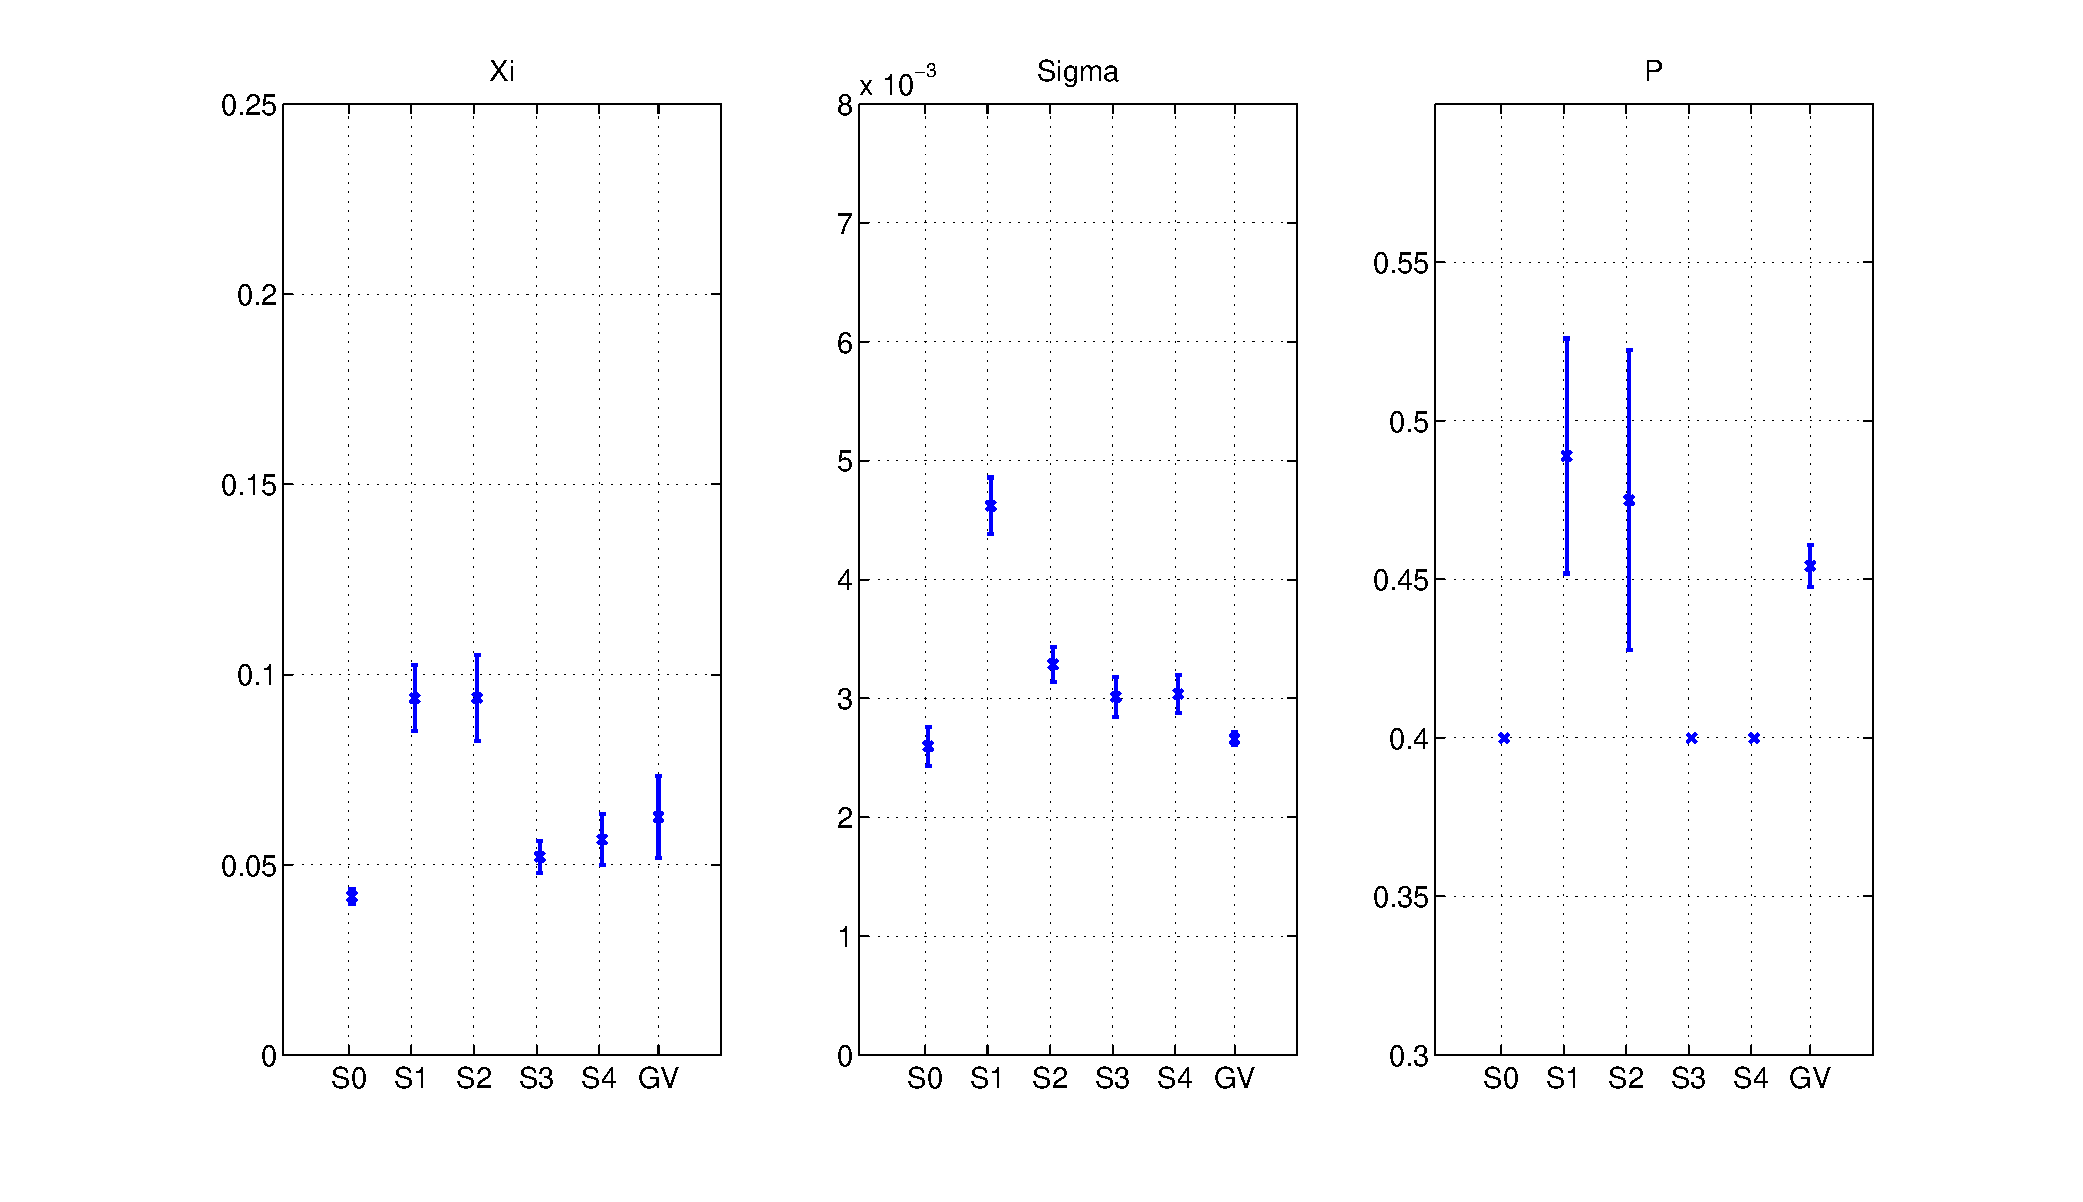
\includegraphics[width=1\textwidth]{images/results/localview/session_experiment/20sessions}
	}
	\caption{Session experiment for the Local View model (II). Different session cases using the same traffic configuration for flow number and flow inter-arrivals.}
	\label{fig:lv_session_exp2}
\end{figure}

It can be observed how for higher loads (see 20 and 15 session cases), the local estimated parameters fit better with the global ones than those cases with a lower load. It is possible to conclude from this experiment, that the load affects the estimation process of the local parameters. For a higher load, the sensors may be able to obtain more samples, which will lead to a closer estimation of the local parameters to the ones in the Global View model as it has been presented in the results of this section.

\clearpage
\section{Load Experiment - Results} \label{sec:lv_load_results}
In the session experiment (Section \ref{sec:lv_load_results}) we tested the effect of different number of sessions, representing different load cases in the estimation and validation process of the local view model. In the experiment presented in this section, we tested the effect of the load over the local view model. We studied two different load cases for two different number of sessions as follows:

\begin{itemize}
	\item 8 sessions - $\approx$ 25 \% load
	\item 15 sessions - $\approx$ 25 \% load
	\item 8 sessions - $\approx$ 35 \% load
	\item 15 sessions - $\approx$ 35 \% load
\end{itemize}

The traffic configuration follows the same parametrization presented in Table \ref{table:lv_traffic}. The user realization for this experiment is presented in Figure \ref{fig:lv_user_realization2}.

\begin{figure}[h!]
	\centering
	\subfloat[8 sessions]{
		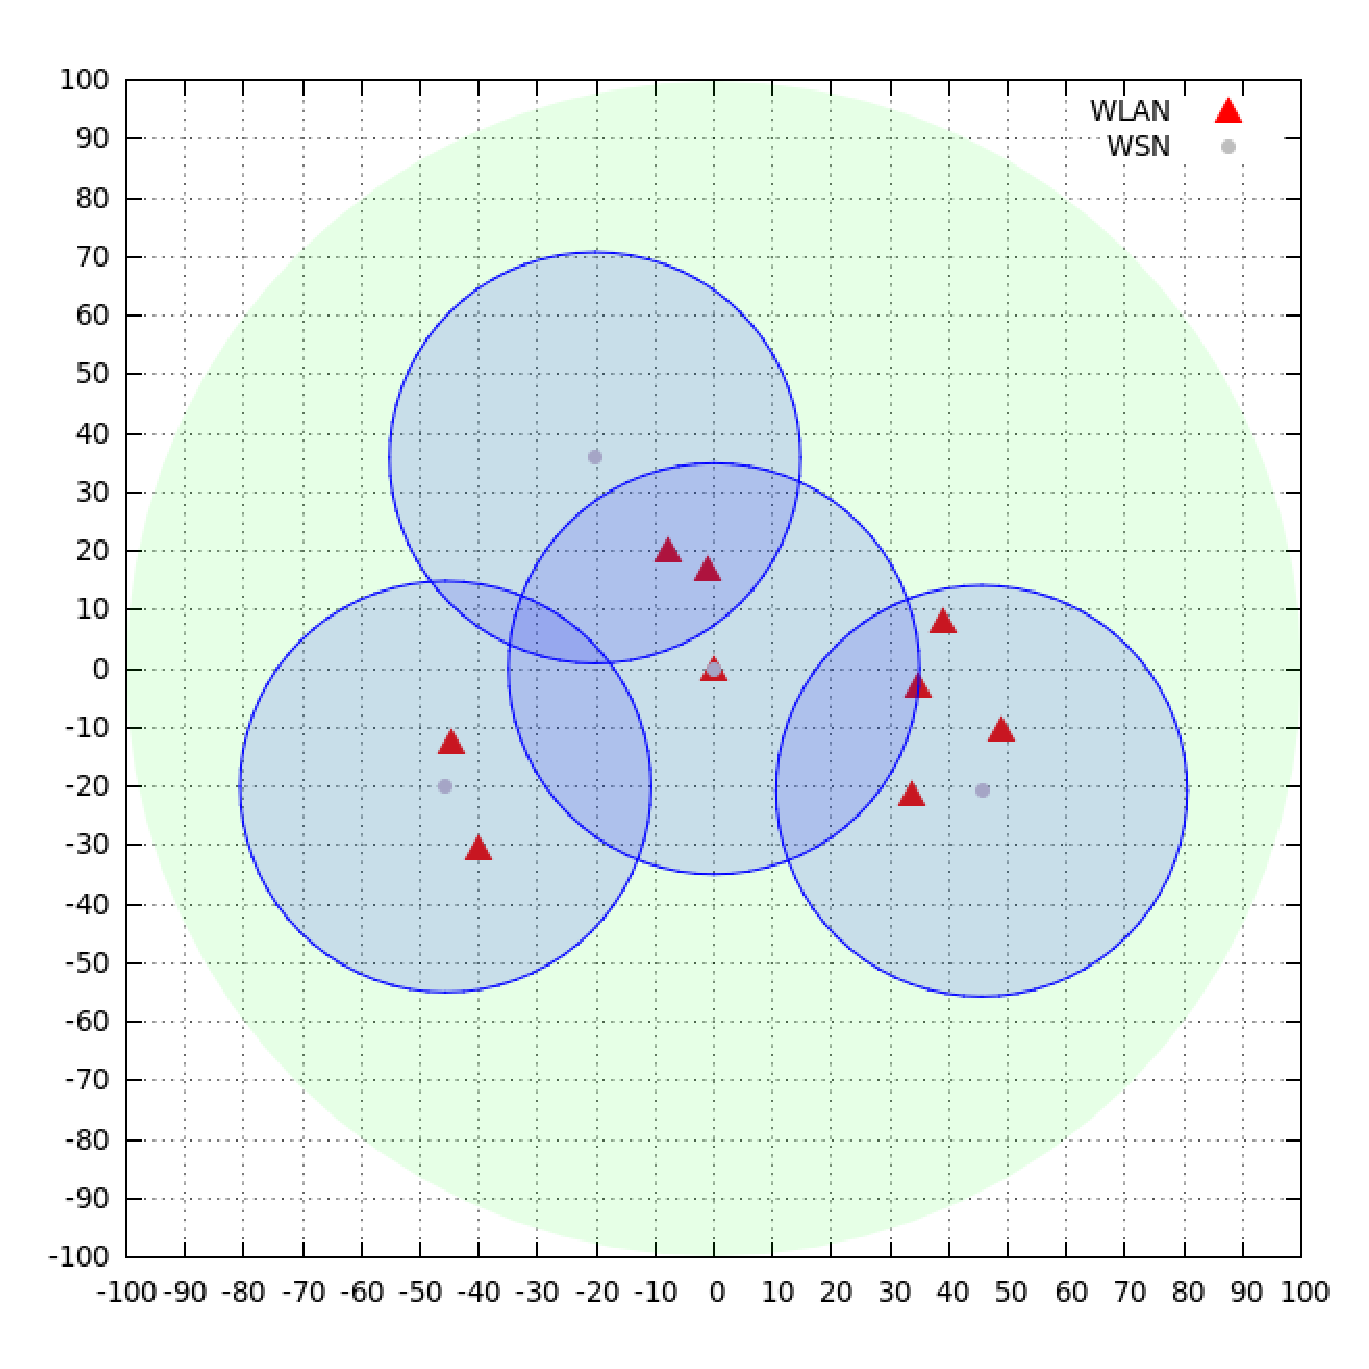
\includegraphics[width=0.5\textwidth]{images/results/localview/load_experiment/8sessions_3sensors}
	}
	\subfloat[15 sessions]{
		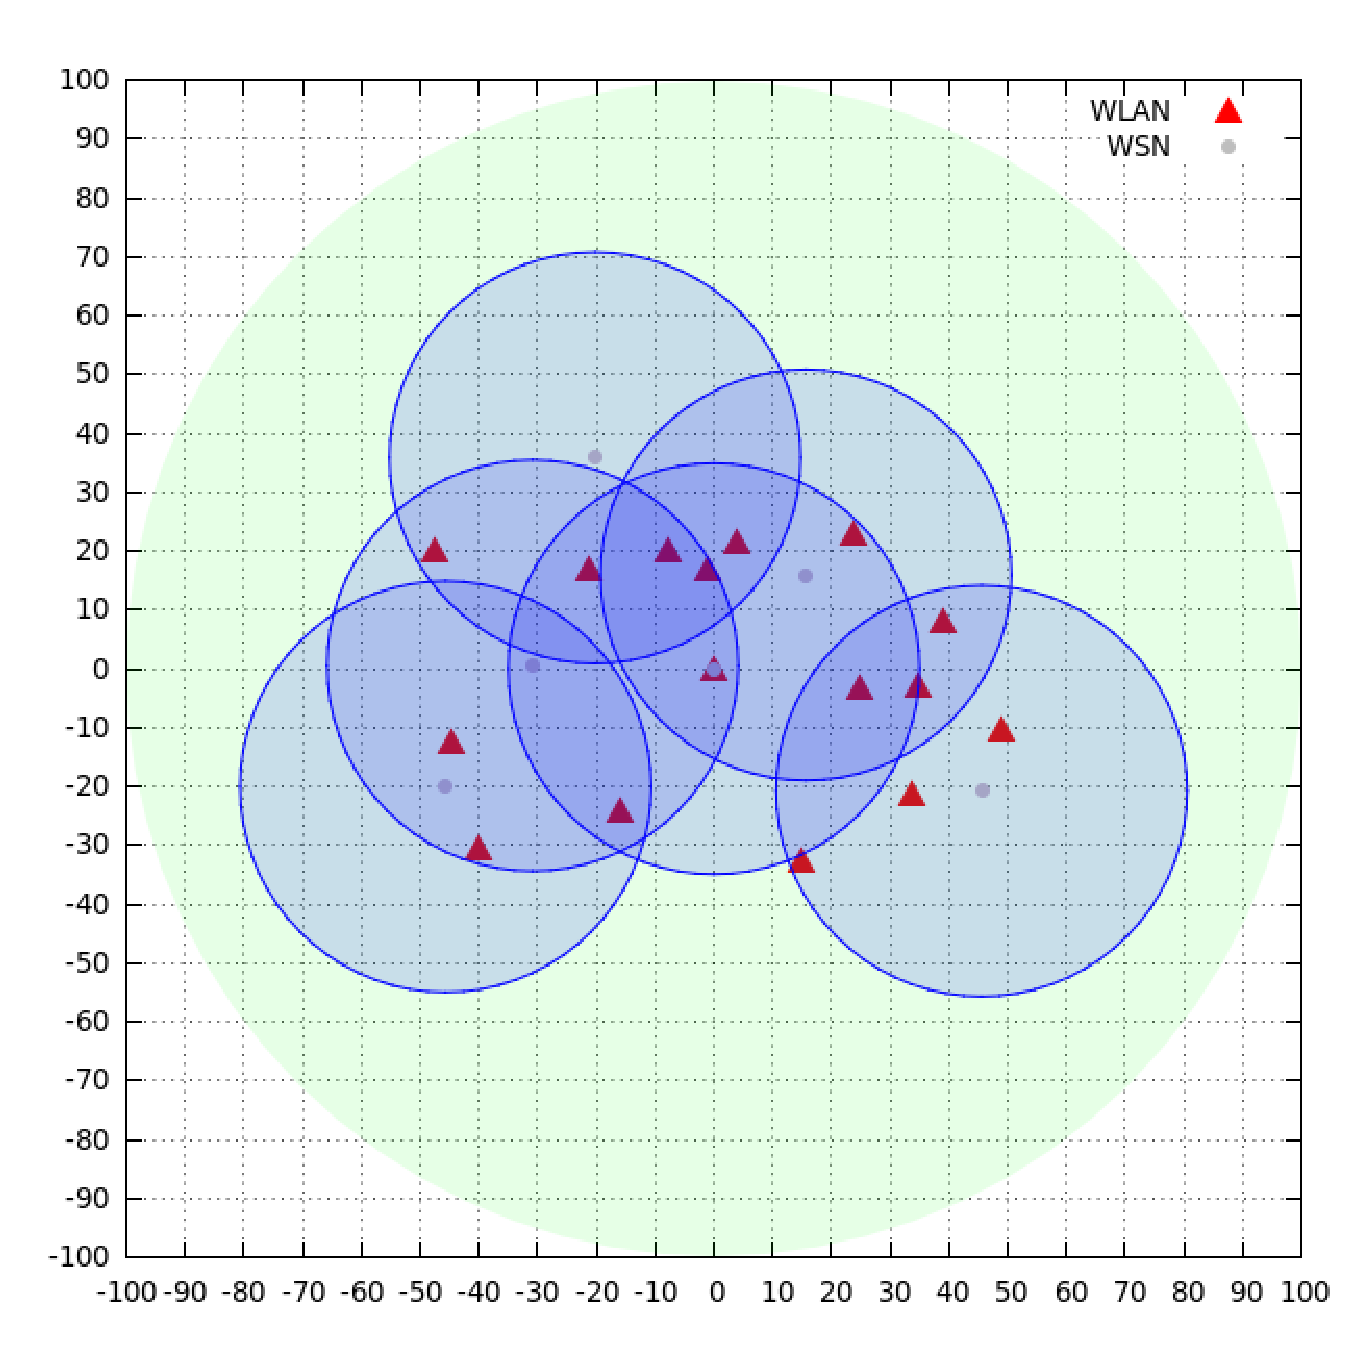
\includegraphics[width=0.5\textwidth]{images/results/localview/session_experiment/15sessions_5sensors}
	}
	\caption{User realization for the Local View load experiment}
	\label{fig:lv_user_realization2}
\end{figure}

The main goal of this experiment is to compare two different load cases for two different number of sessions and observe how this affects the estimation process of the Local View model.

The results obtained for this experiment are represented in Figures \ref{fig:lv_load_exp1} and \ref{fig:lv_load_exp2}. Figure \ref{fig:lv_load_exp1} represents a low-medium load case for two different number of users. As it can be observed from the estimated parameters, the higher is the number of sessions, more close are the estimated local parameters to the ones of the Global View model. In Figure \ref{fig:lv_load_exp2} we present a higher load case. Although there is still a small improvement in the 15 session case, both session cases present a similar behaviour in the estimation process when the load is higher.

\begin{figure}[h!]
	\centering
	\subfloat[8 sessions - $\approx$ 25 \% load]{
		\label{fig:lv_8_25}
		\includegraphics[width=1\textwidth]{images/results/localview/load_experiment/8sessions_25load_2}
	}\\
	\subfloat[15 sessions - $\approx$ 25 \% load]{
		\label{fig:lv_15_25}
		\includegraphics[width=1\textwidth]{images/results/localview/load_experiment/15sessions_25load_2}
	}
	\caption{Load experiment for the Local View model (I). Different number of sessions with similar load.}
	\label{fig:lv_load_exp1}
\end{figure}

\begin{figure}[h!]
	\centering
	\subfloat[8 sessions - $\approx$ 35 \% load]{
		\label{fig:lv_8_35}
		\includegraphics[width=1\textwidth]{images/results/localview/load_experiment/8sessions_35load_2}
	}\\
	\subfloat[15 sessions - $\approx$ 35 \% load]{
		\label{fig:lv_15_35}
		\includegraphics[width=1\textwidth]{images/results/localview/load_experiment/15sessions_35load_2}
	}
	\caption{Load experiment for the Local View model (II). Different number of sessions with similar load.}
	\label{fig:lv_load_exp2}
\end{figure}

From the results presented in this section, we can conclude from this experiment that the estimation process is better for a higher number of sessions when the load is low-medium. On the other hand, the estimation process is not improved significantly by the number of sessions for higher loads.